\chapter{Cloud Security with Honeypots}

\section{Introduction}

As previously mention in \fullref{sec:cloud-computing}, using cloud resources are becoming the go-to option for new services, and applications.
\citet{Kelly2021} thoroughly investigated honeypots on cloud providers such as Azure, AWS, or Goolge Cloud Platform.
Followingly, we present their results that we want to compare with the results of HeiCLOUD later on.
The results are collected by T-Pot version 20. over a duration of 3 weeks with 24h per day.
A detailed describtion of T-Pot is done in \fullref{sec:tpot}.
In addition, \citet{Kelly2021} considered different server geographical locations.
They have collected data from East US, West Europe, Southeast Asia.
\autoref{tab:overview-cloud-security} shows the results presented by \citet{Kelly2021}.
Dionaea, Cowire, and Conpot are the most attacked honeypots in comparison to the others.
Regarding \ac{aws}, Dionaea account $91\%$ of the total attacks, Glutton and Cowire are minor with $5\%$, and $2\%$.
Interestingly, Cowire reported several attacks related to the COVID-19 pandamic to enable social engineering methods.
In contrast to \ac{aws}, Cowire logged the majority of attacks with $51\%$ on \ac{gc}.
Beside several automated attacks trying to login with default credentials, adversaries tried to gather information about CPU architecture, scheduled tasks, and privilege escalation.
Microsoft Azure reflects nearly the same results as the two other cloud providers beforehand.

\begin{table}[h]
    \centering
    \caption[Overview of attacks on cloud providers]{Overview of attacks on cloud providers. For a better overview, only the three most attacked honeypots are listed. The others combine several honeypots.}
    \begin{tabular}{l|llll|l}
        \toprule
        \textbf{Provider} & \multicolumn{4}{c|}{\textbf{Honeypot}} & \textbf{In Total}                                   \\
                          & Dionaea                               & Cowire            & Glutton  & others   &           \\
        \hline
        \acl{aws}         & $228.075$                             & $4.503$           & $11.878$ & $3.688$  & $248.144$ \\
        \acl{gc}          & $162.570$                             & $297.818$         & $84.375$ & $36.403$ & $581.116$ \\
        Microsoft Azure   & $308.102$                             & $9.012$           & $17.256$ & $6.365$  & $340.735$ \\
        \bottomrule
    \end{tabular}
    \label{tab:overview-cloud-security}
\end{table}

The overall results show a average attack ratio of $55.000$ per day, summing up to roughly $1.6$mio attacks. 
In total, the most attacking countries are China, 

\section{HeiCLOUD}

\citet{urz2021} offers a \enquote{\ac{iaas} specially tailored for higher education and research institutions} called heiCLOUD.
It supplies multiple institutes at University Heidelberg with storage, virtual machines, or network components.
In addition, heiCLOUD is a DFN\footnote{German National Research and Education Network,  the communications network for Science and research in Germany} member, and offers others to use their services.
As stated on their information website\cite{heicloud2021}, it is
\begin{enumerate*}[label=(\roman*)]
    \item capable of freely manageable IT resources,
    \item beholds a stable and fast connection,
    \item ensures high availability and scalability,
    \item has freely selectable VM operating systems, and
    \item has a transparent payment model
\end{enumerate*} \cite{heicloud2021}.
Based on the open source application OpenStack, users can easily create own network areas, and manage their space individually.
Unlike well-known cloud providers, heiCLOUD servers are located withing Germany, thus, abide by the European data privacy law.
HeiCLOUD have never considered honeypots for additional cyber security measurements whereas other cloud providers developed advanced structures.
In \fullref{sec:honeypots-heicloud}, we show various results of honeypots in heiCLOUD, stress out the importance of it, and lay emphasis on our concept in \autoref{chap:concept}.

\section{T-Pot}
\label{sec:tpot}

T-Pot is a hollistic approach to capture recent cyber attacks by the sheer quantity of various honeypots.
The German IT provider Telekom
In conjucntion with a
For this thesis we restrict ourself to the latest version 20.06.0. Newer versions might differ from this one.

\subsection{Honeypots}

Due to the sheer quantity of honeypots we want to give some basic knowledge about them. \autoref{tab:overview-honeypots} gives a quick overview of all available honeypots in conjunction with the port they are running on, service , and a short decription.

\textbf{ADBHoney} \cite{adbhoney2021} is a low interaction \ac{adb} honeypot over TCP/IP.
The importance of this honeypot lies in the \ac{adb} protocol that is used to debug and push content to the device.
However, unlike USB it does not support any kind of ample mechanisms of authentication and protection.
By exposing the \ac{adb} service over any port, any adversary could connect and exploit this device.
ADBHoney is designed to catch malware that has been pushed onto the device.

\textbf{Cisco \ac{asa}} \cite{cymmetria2018} is a low interaction honeypot that detects CVE-2018-0101\cite{CVE-2018-0101}.
It is a vulnerability that could allow an unauthenticated, remote attacker to cause a reload of the affected system or to remotely execute code.
This can be achieved by flooding a webvpn-configured interface with crafted XML packets.
Consequently, the attacker obtain full control by executing arbitrary code.

\textbf{Citrix \ac{adc} honeypot} \cite{citrixhoneypot2020} detects and logs CVE-2019-19781\cite{CVE-2019-19781} scan and exploitation attempts.
This vulnerability allows adversaries to perform directory traversal attacks.
Files are accessible by path strings to denote the file or directory.
In addition, some file systems include special character to easily traverse the hierarchy.
Attackers take advantage of it by combining special characters in order to get access to restricted areas. \cite{flanders2019}

\textbf{Conpot} \cite{conpot2021} is a low interaction industrial honeypot for \ac{ics}, and \ac{scada}.
It provides a variety of different common industrial control protocols.
An adversary should be tricked by the complex infrastructure, and lure him into attacks.
In addition, a custom human machine interface can be conntected to increase the attack surface.
By randomly delaying the response time, conpot tries to emulate a real machine handling a certain amount of load.

\textbf{Cowrie} \cite{cowire2021} is a medium to high interaction SSH and Telnet honeypot.
It offers to log brute-force attacks and shell interactions with attacker.
In medium interaction mode cowire emulates a UNIX shell in Python, whereas in high interaction mode it proxies all commands to another system.

\textbf{DDoSPot} \cite{ddosspot2021} is a low interaction honeypot to log and detect UDP-based \ac{ddos} attacks.
It is used as a platform to support various plugins for different honeypot services, and servers.
Currently, it supports DNS, NTP, SSDP, CHARGEN, and random/mock UDP server.

\textbf{Dicompot} \cite{dicompot2021} is a low interaction honeypot for the \ac{dicom} protocol.
As other honeypots before, it mocks a \ac{dicom} server in Go to collect logs and detect attacks.

\textbf{Dionaea} \cite{dionaea2021} is a medium interaction honeypot that tries to capture malware copies by exposing services.
It supports a vast variety of protocols such as FTP, SMB, and HTTP.
Several modules can be integrated to work with Dionaea such as VirusTotal for further malware results.

\textbf{Elasticpot} \cite{elasticpot2021} is a low interaction honeypot for elasticsearch, a search engine based on the Lucene library.

\textbf{Endlessh} \cite{endlessh2021} is a SSH server that sends an endless, random SSH banner.
The key idea is to lock up SSH clients that try to connect to the SSH server.
It lowers to transcation speed by intentionally inserting delays.
Due to connection establishing before cryptographic exchange, this module does not require any cryptographic libraries.

\textbf{Glutton} \cite{glutton2021} is a generic low interaction honeypot that works as a MitM for SSH and TCP.
However, lacking documentation does not provide a deeper inside of this honeypot.

\textbf{Heralding} \cite{heralding2021} is a credential catching honeypot for protocols like FTP, Telnet, SSH, HTTP, or IMAP.

\textbf{HellPot} \cite{hellpot2021} is a \enquote{endless honeypot}.
Connecting to this honeypot results in a memory overflow.
Its key idea is to send an endless stream of data to the attacker until its memory, or storage runs out.

\textbf{HoneyPy} \cite{honeysap2021} is a low to medium interaction honeypot that supports several protocols such as UDP, or TCP.
New protocols can be added by writing a custom plugin for it.
HoneyPy should give the freedom of easily deploying and extending honeypots.

\textbf{HoneySAP} \cite{honeysap2021} is a low interaction honeypot tailored for SAP services.

\textbf{HoneyTrap} \cite{honeytrap2021} is a low interaction honeypot network security tool
As stated by \citet*{honeytrap2021}, HoneyTrap is vulnerable by buffer overflow attacks.

\textbf{IPPHoney} \cite{ipphoney2021}

\textbf{Mailoney} is an SMTP honeypot.

\textbf{MEDpot} \cite{medpot2021}

\textbf{RDPY} \cite{rdpy2021} is a low interaction honeypot of the Microsoft \ac{rdp} written in Python.
It features client and server side, and it based on the event driven network engine Twisted.
It supports authentication over SSL and NLA.

\textbf{RedisHoneyPot} is a high interation honeypot for Redis protocol written in Go.

\textbf{SNARE} \cite{snare2021} is an abbreviation for Super Next generation Advanced Reactive honEypot.
It is a successor of Glastopf, a web application sensor.
In addition, it supports the feature of converting existing webpages into attack surfaces.

\textbf{TANNER} \cite{tanner2021} can be seen as SNARES's brain.
Whenever has been sent to SNARE, TANNER decides how the response should like.

\begin{table}[h]
    \centering
    \caption[Overview honeypots of T-Pot]{Overview of all available honeypots of T-Pot in conjunction with the service level. In addition, }
    \begin{tabularx}{\linewidth}{l|l|l}
        \toprule
        \textbf{Honeypot}                        & \textbf{Description} & \textbf{Port} \\
        \hline
        adbhoney                                 &                      &               \\
        ciscoasa \cite{cymmetria2018}            &                      &               \\
        citrixhoneypot \cite{citrixhoneypot2020} &                      &               \\
        conpot \cite{conpot2021}                 &                      &               \\
        cowrie \cite{cowire2021}                 &                      &               \\
        ddospot \cite{ddosspot2021}              &                      &               \\
        dicompot \cite{dicompot2021}             &                      &               \\
        dionaea \cite{dionaea2021}               &                      &               \\
        elasticpot \cite{elasticpot2021}         &                      &               \\
        endlessh \cite{endlessh2021}             &                      &               \\
        glutton \cite{glutton2021}               &                      &               \\
        heralding \cite{heralding2021}           &                      &               \\
        hellpot \cite{hellpot2021}               &                      &               \\
        honeypy \cite{honeysap2021}              &                      &               \\
        honeysap \cite{honeysap2021}             &                      &               \\
        honeytrap \cite{honeytrap2021}           &                      &               \\
        ipphoney \cite{ipphoney2021}             &                      &               \\
        mailoney                                 &                      &               \\
        medpot \cite{medpot2021}                 &                      &               \\
        rdpy \cite{rdpy2021}                     &                      &               \\
        redishoneypot                            &                      &               \\
        snare \cite{snare2021}                   &                      &               \\
        tanner \cite{tanner2021}                 &                      &               \\
        \bottomrule
    \end{tabularx}
    \label{tab:overview-honeypots}
\end{table}

\subsection{Tools}

In addition, T-Pot integrates following tools to investigate and handle network traffic:

\begin{itemize}
    \item Cockpit
    \item Cyberchef
    \item ELK stack
    \item Elasticsearch head
    \item Fatt
    \item Spiderfoot
    \item Suricata
\end{itemize}

\subsection{Workflow}

\autoref{fig:overview-tpot} shows the connection between all components.

\begin{sidewaysfigure}[h]
    \centering
    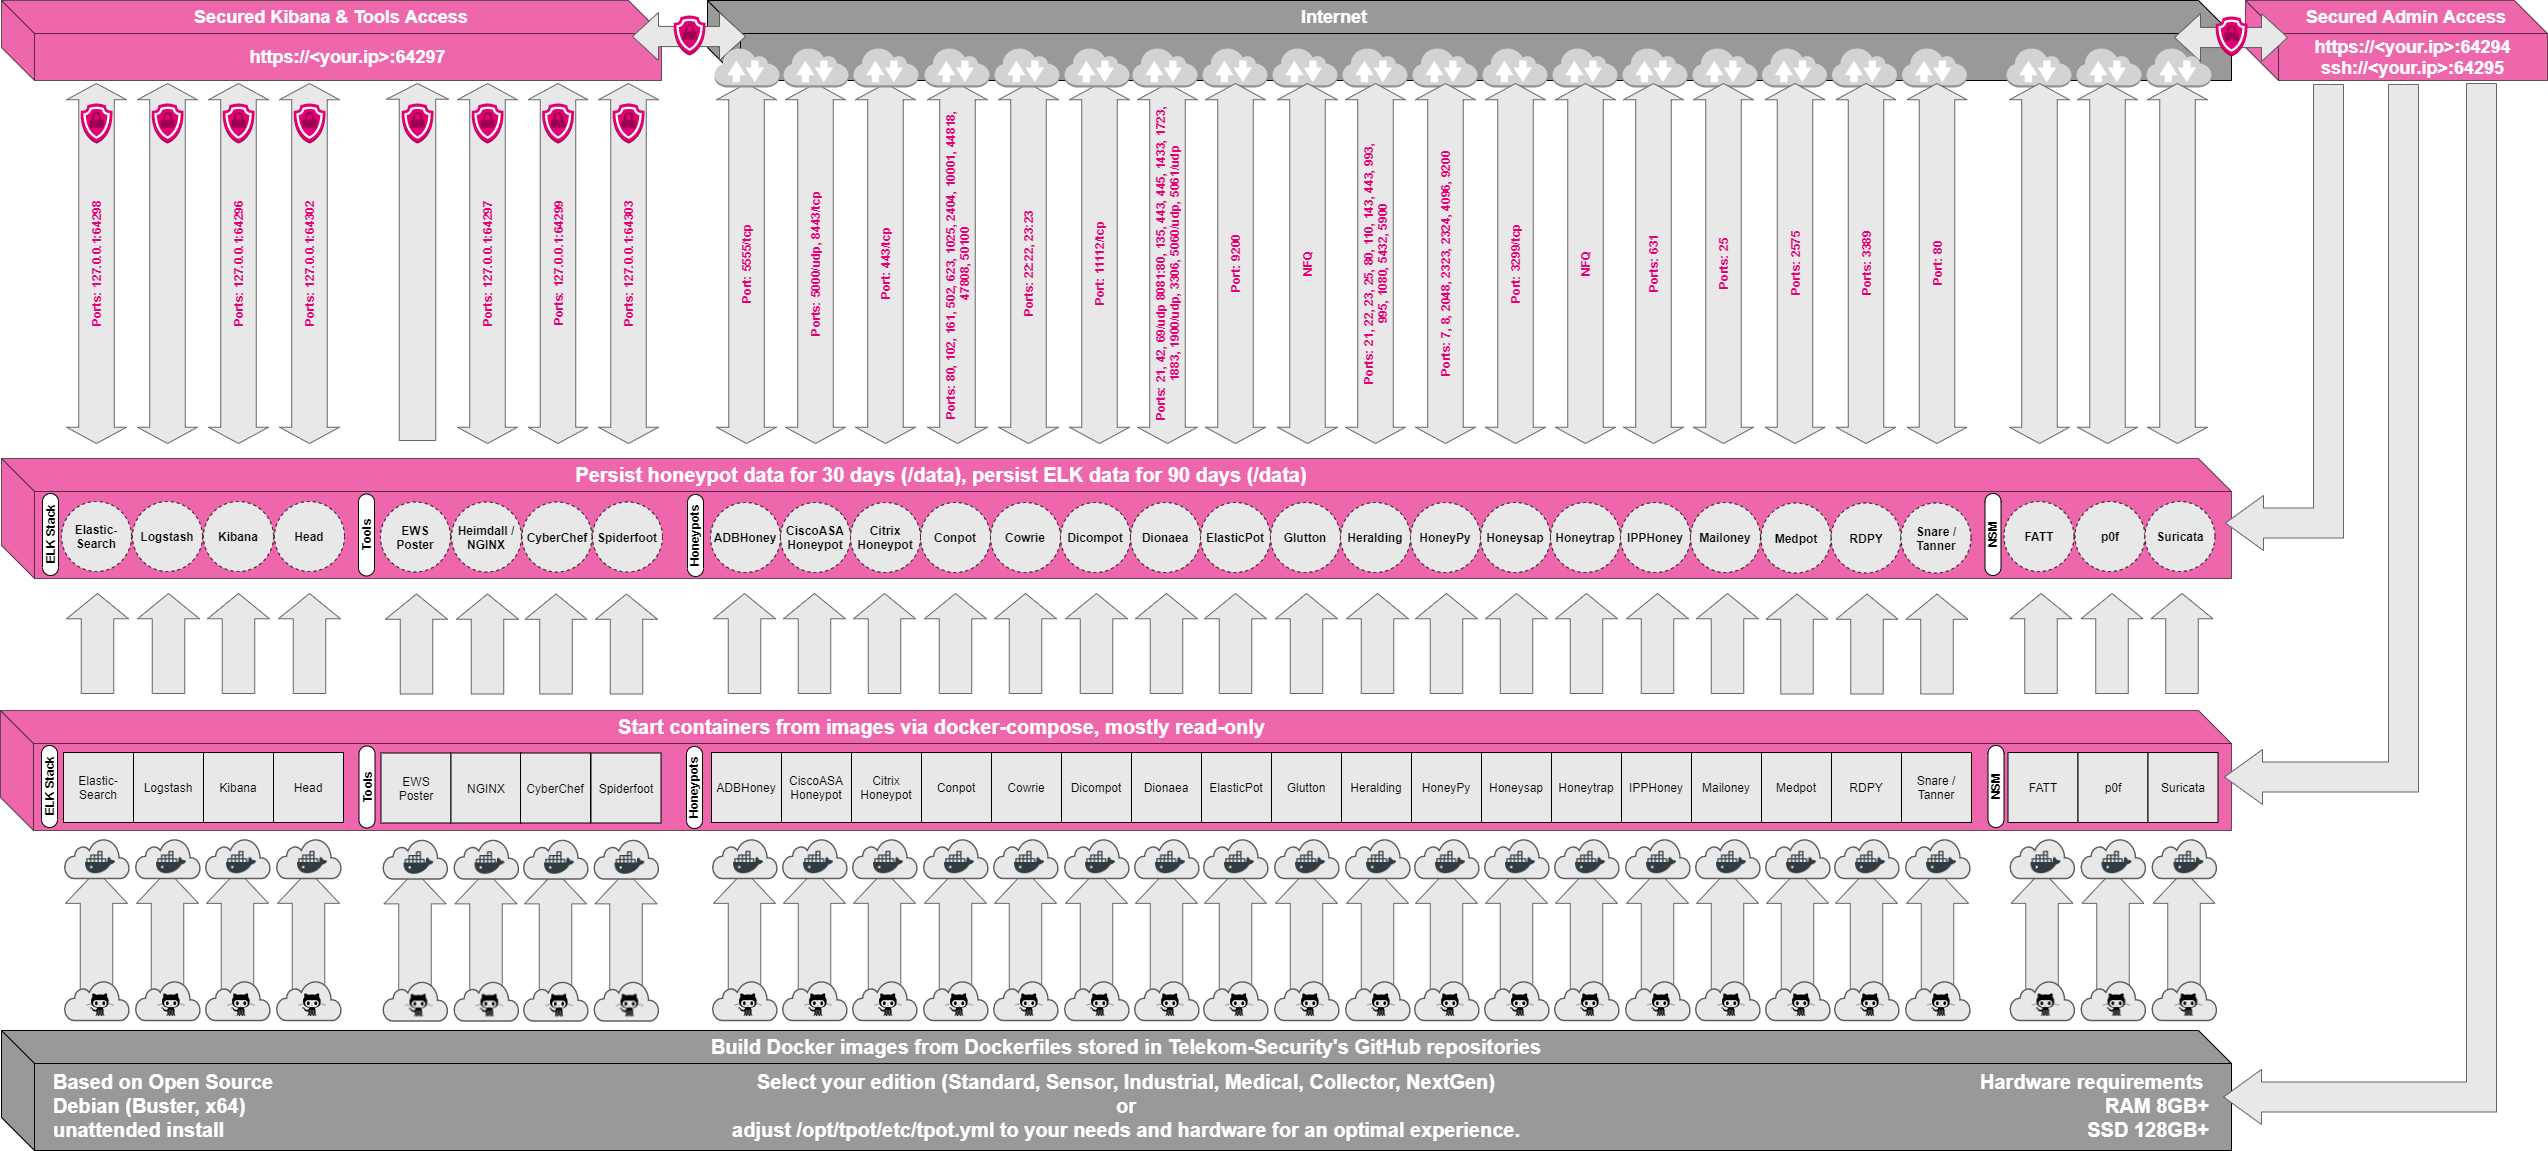
\includegraphics[width=\textwidth]{figures/architecture.png}
    \caption{}
    \label{fig:overview-tpot}
\end{sidewaysfigure}

\section{Data Analysis}

\citet{NawrockiWSKS2016} have done a sophisticated survey of honeypots and data analysis.
Based on their findings we give a short summary of the honeypot data analysis.

\begin{enumerate}
    \item Attack Profile
    \item Attack Source
    \item Attack Target
    \item Attack Frequency
    \item Attack Evolution
    \item Propagation of Attacks
    \item Attack Patterns
    \item Attack Root Cause Identification
    \item Attack Risk Assessment
    \item Exploit Detection
\end{enumerate}

\todo{übersicht tabelle}
\begin{table}[h]
    \centering
    \caption{}
    \begin{tabularx}{\linewidth}{l}
        \toprule
        Attack Profile                   \\
        Attack Source                    \\
        Attack Target                    \\
        Attack Frequency                 \\
        Attack Evolution                 \\
        Propagation of Attacks           \\
        Attack Patterns                  \\
        Attack Root Cause Identification \\
        Attack Risk Assessment           \\
        Exploit Detection                \\
        \bottomrule
    \end{tabularx}
    \label{tab:overview-data-analysis}
\end{table}


\section{Honeypots in HeiCloud}
\label{sec:honeypots-heicloud}

\todo{verwendung von Grafiken, etc.}

\subsection{Overview}

\subsection{SSH}

\subsection{Malware Capturing}



\todo{show results}

Despite the amount of honeypots, we restrict ourself to consider only a few honeypots.
Reason for that is the \fullref{chap:concept}

\section{Summary}

In this chapter we have